\documentclass[]{article}
\usepackage{xcolor}
\usepackage{amsmath}
\usepackage{graphicx}


%opening
\title{MTH 343 Numerical Analysis Lecture 6: Secant Method}
\author{Sheikh Abdul Raheem Ali}

\begin{document}
	\newcommand{\cfbox}[2]{%
		\colorlet{currentcolor}{.}%
		{\color{#1}%
			\fbox{\color{currentcolor}#2}}%
	}

\maketitle

Suppose \cfbox{red}{f(x) = 0}

\section*{Technique:}

\begin{enumerate}
	\item Begin with two values $ x_0 $ \& $ x_1 $ near the root $ r $. Draw a line joining the two points. The point $ x_2 $ where this line hits the x-axis is the first approximation of the exact root $ r $. 
	\item Continue this repeatedly, always choosing the last computed values for drawing this straight line. 
\end{enumerate}

\section*{Derivation:}

\begin{align*}
	\frac{y-y_1}{x-x_1} = m \text{ or } y - y_1 = m(x - x_1)s\\
	\frac{y - f(P_1)}{x-P_1} &= \frac{f(P_1) - f(P_0)}{P_1 - P_0}\\
	 y &= f(P_1) + \frac{f(P_1) - f(P_0)}{P_1 - P_0}(x - P_1)\\
	\text{To find x-intercept, set y=0},\\
	0 &= f(P_1) + \frac{f(P_1)-f(P_0)}{P_1 - P_0}(x-P_1)\\
	0 &= f(P_1)(P_1-P_0) + (f(P_1) - f(P_0))(x - P_1)\\
	(f(P_1)-f(P_0))(x-P_1) &= - f(P_1)(P_1 - P_0)\\
	x &= P_1 - \frac{f(P_1)(P_1 - P_0)}{f(P_1) - f(P_0)}\\
	P_2 &= P_1 - \frac{f(P_1)(P_1 - P_0)}{f(P_1) - f(P_0)}
\end{align*}

\section*{Example:}

\[ f(x) = x^2 - 2 \]

%A dirty hack to get the table centered
\begin{enumerate}
	\item[]
	\centering
	\begin{tabular}{c c c}
		$ n $ & $ P_{n} $ & $ f(P_n) $ \\
		2&1.6&0.56\\
		3&1.47826&0.18525\\
		4&1.418079&0.01094\\
		5&1.414299&0.000241 
	\end{tabular}
\end{enumerate}

\section*{Disadvantages of the Secant Method}

\begin{enumerate}
	\item If the fraction is far from linear near the root, the iterates can fly off to points far from the root. This can be fixed by plotting $ f(x) $ and changing the starting points.
	
	\item If an iterate duplicates a previous one this results in an endless loop that never reaches the value of the true solution.
	
	\item Secant method doesn't have the bracketing property of the bisection method. Therefore, the method doesn't always converge. But if it does, it is generally faster than the bisection method.
\end{enumerate}


\begin{figure}[h!]
	\centering
	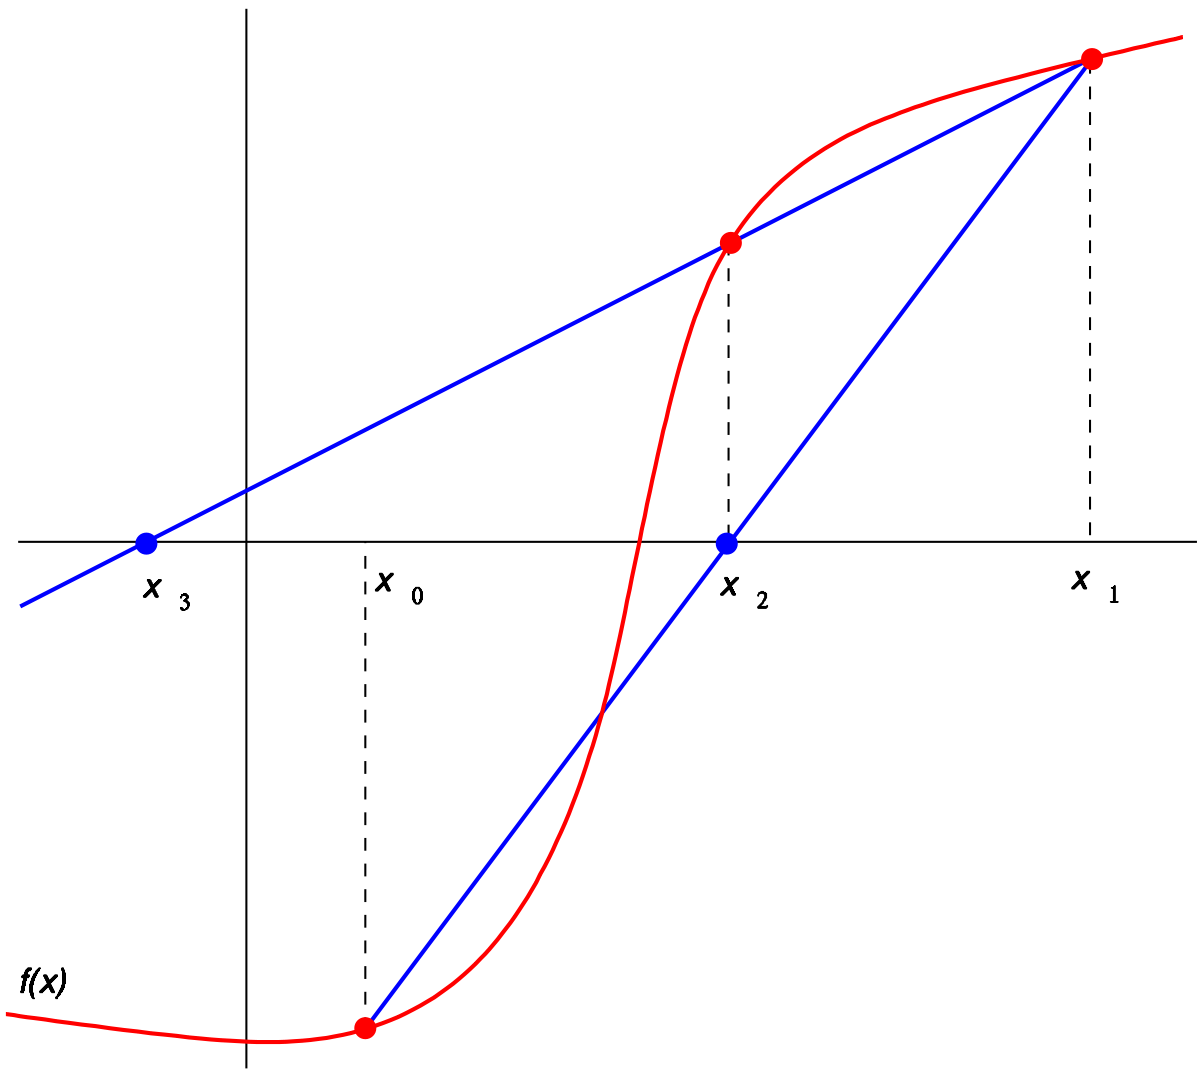
\includegraphics[width= 0.8\linewidth]{secant.png}
	\caption{Visual demonstration of the secant method}
\end{figure}

\end{document}
